\begin{problem}[问题6.7]
$Z$平面上, 宽$a$的无限长狭缝, 对称中心存在强度为$Q$的点源, 求复速度势.
\end{problem}
\begin{solution}
\textbf{解:} 图\ref{p7f1}为保角变换坐标轴示意图, 图\ref{p7f2}为变换前后对应点的关系.
\begin{figure}[!htb]
\begin{minipage}[b]{.65\textwidth}
\centering
\usetikzlibrary{%
    decorations.pathreplacing,%
    decorations.pathmorphing,arrows
}
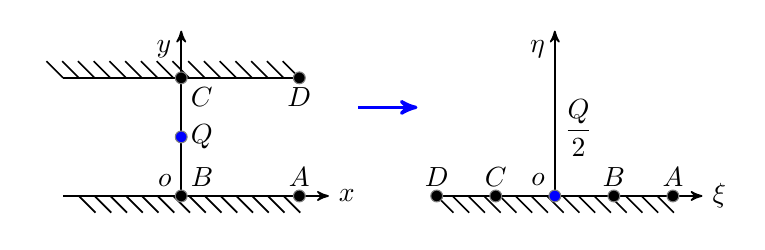
\begin{tikzpicture}[ media/.style={font={\footnotesize\sffamily}},
    interface/.style={
        postaction={draw,decorate,decoration={border,angle=-45,
                    amplitude=0.3cm,segment length=2mm}}},scale=1.5]
%\draw(0.7,-0.22) rectangle (6.7,1.425);
\clip(0.7,-0.22) rectangle (6.7,1.425);
\draw[semithick,interface](3,1)--(1,1) (1,0)--(3,0) ;
\draw[semithick,->,>=stealth'](3,0)--(3.25,0) node[right]{$x$};
\draw[semithick,->,>=stealth'](2,0)--(2,1.4) node[below left]{$y$};
\fill[black,draw=gray](2,0) circle(0.05) node[above left]{$o$} node[above right]{$B$};
%\draw[semithick,dashed,blue](1,0)--(3,0.8284);

\fill[blue,draw=gray](2,0.5) circle(0.05) node[right,black]{$Q$};

\fill[black,draw=gray](3,0) circle(0.05) node[above]{$A$};


\fill[black,draw=gray](2,1) circle(0.05) node[below right]{$C$};
\fill[black,draw=gray](3,1) circle(0.05) node[below]{$D$};


\draw[very thick,blue,->,>=stealth'](3.5,0.75)--(4,0.75);

\begin{scope}[xshift=90]
\draw[semithick,interface](1,0)--(3,0);
\draw[semithick,->,>=stealth'](3,0)--(3.25,0) node[right]{$\xi$};
\draw[semithick,->,>=stealth'](2,0)node[above left]{$o$}--(2,1.4) node[below left]{$\eta$};
\fill[blue,draw=gray](2,0) circle(0.05); 
\node at (2.2,0.25)[above,black]{$\displaystyle\frac{Q}{2}$};
\fill[black,draw=gray](2.5,0) circle(0.05) node[above,black]{$B$};
\fill[black,draw=gray](3,0) circle(0.05) node[above,black]{$A$};

\fill[black,draw=gray](1.5,0) circle(0.05) node[above,black]{$C$};
\fill[black,draw=gray](1,0) circle(0.05) node[above,black]{$D$};

\end{scope}
\end{tikzpicture}

\vspace{-0.25em}
\caption{\label{p7f1}保角变换示意图}
\end{minipage}%
\begin{minipage}[b]{.35\textwidth}
\centering
\begin{tabular}{l|lll}
\multicolumn{1}{c|}{} & \multicolumn{1}{c}{$z$} & \multicolumn{1}{c}{$\alpha_i$} & \multicolumn{1}{c}{$a_i$} \\
\hline
\multicolumn{1}{c|}{A} & \multicolumn{1}{c}{$\infty$} & \multicolumn{1}{c}{$\pi$} & \multicolumn{1}{c}{$\infty$} \\
\multicolumn{1}{c|}{B} & \multicolumn{1}{c}{$0$} & \multicolumn{1}{c}{$\pi/2$} & \multicolumn{1}{c}{1} \\
\multicolumn{1}{c|}{C} & \multicolumn{1}{c}{$ai$} & \multicolumn{1}{c}{$\pi/2$} & \multicolumn{1}{c}{-1} \\
\multicolumn{1}{c|}{D} & \multicolumn{1}{c}{$\infty+ai$} & \multicolumn{1}{c}{$\pi$} & \multicolumn{1}{c}{$-\infty$} \\
\end{tabular}
\caption{\label{p7f2}变换前后对应点的关系}
\end{minipage}
\end{figure}

\noindent 如图\ref{p7f1}所示, 将无穷带域的右半部分用Schwarz-christoffel变换为上半平面
\begin{eqnarray}
\frac{dz}{d\zeta} &=& K\Pi_{i=1}^N(\zeta-a_i)^{\beta_i}, {~~} \beta_i = \frac{\alpha_i}{\pi}-1\nonumber\\
&=& K(\zeta+1)^{-1/2}(\zeta-1)^{-1/2}\nonumber\\
&=& K(\zeta^2-1)^{-1/2}\nonumber
\end{eqnarray}
积分可得$z=K\cosh^{-1}\zeta$或$\zeta=\cosh \frac{z}{K}$,由$A,B,C,D$得$K=a/\pi$, 代入$Q$点
\[
\zeta_0 = \cosh\frac{\pi}{a}\frac{ia}{2} = 0
\]
又由镜像法可得$\xi-\eta$平面上的复速度势
\[
W(\zeta) = \frac{Q/2}{2\pi}\ln(\zeta-\zeta_0) + \frac{Q/2}{2\pi}\ln(\zeta-\overline{\zeta_0}) = \frac{Q}{2\pi}\ln(\zeta)
\]
因此$z$平面上的复速度势
\begin{eqnarray}
W(z) &=& \frac{Q}{2\pi}\ln(\cosh \frac{\pi z}{a})
\end{eqnarray}


\end{solution}

